\chapter{User Documentation}
\label{chap:user-documentation}

This chapter provides user documentation for the CryptoShow application, including a brief introduction on how to use the application.

\section{How to Use}
\label{sec:how-to-use}

To use the CryptoShow application, either deploy it locally (see Section~\ref{sec:deployment}) or access the live version at \url{https://cryptoshow.cz}.

Upon opening the main page, an input table is displayed. Provide either a structure identifier (PDB or AlphaFold ID) or upload a PDB/mmCIF file. Once a valid structure is provided, the application will begin processing and displays the computation status. Processing time varies based on the structure size and server load.

Once the computation is finished, the user is presented with a link to the calculation results. After clicking the link, the user is redirected to the visualization page. The following elements are shown:

\begin{itemize}
    \item An interactive 3D visualization of the structure, allowing users to rotate and zoom. Residues that are part of detected cryptic binding sites are highlighted using distinct colors.
    \item A toolbox providing options to adjust visualization styles.
    \item A table listing the identified cryptic binding sites with expandable rows. Each entry includes details about the involved residues, their scores, and a PyMOL selection string for visualizing the site in PyMOL. For each pocket (in PDB structures), users can initiate an AHoJ query to obtain apo-holo pairs and visualize possible conformational changes. Results can also be downloaded as a ZIP archive.
\end{itemize}

The 3D visualization in Mol* with the toolbox is shown in Figure~\ref{fig:ui-molstar}. The results table with expandable rows is shown in Figure~\ref{fig:ui-table}.

\begin{figure}[htbp]
    \centering
    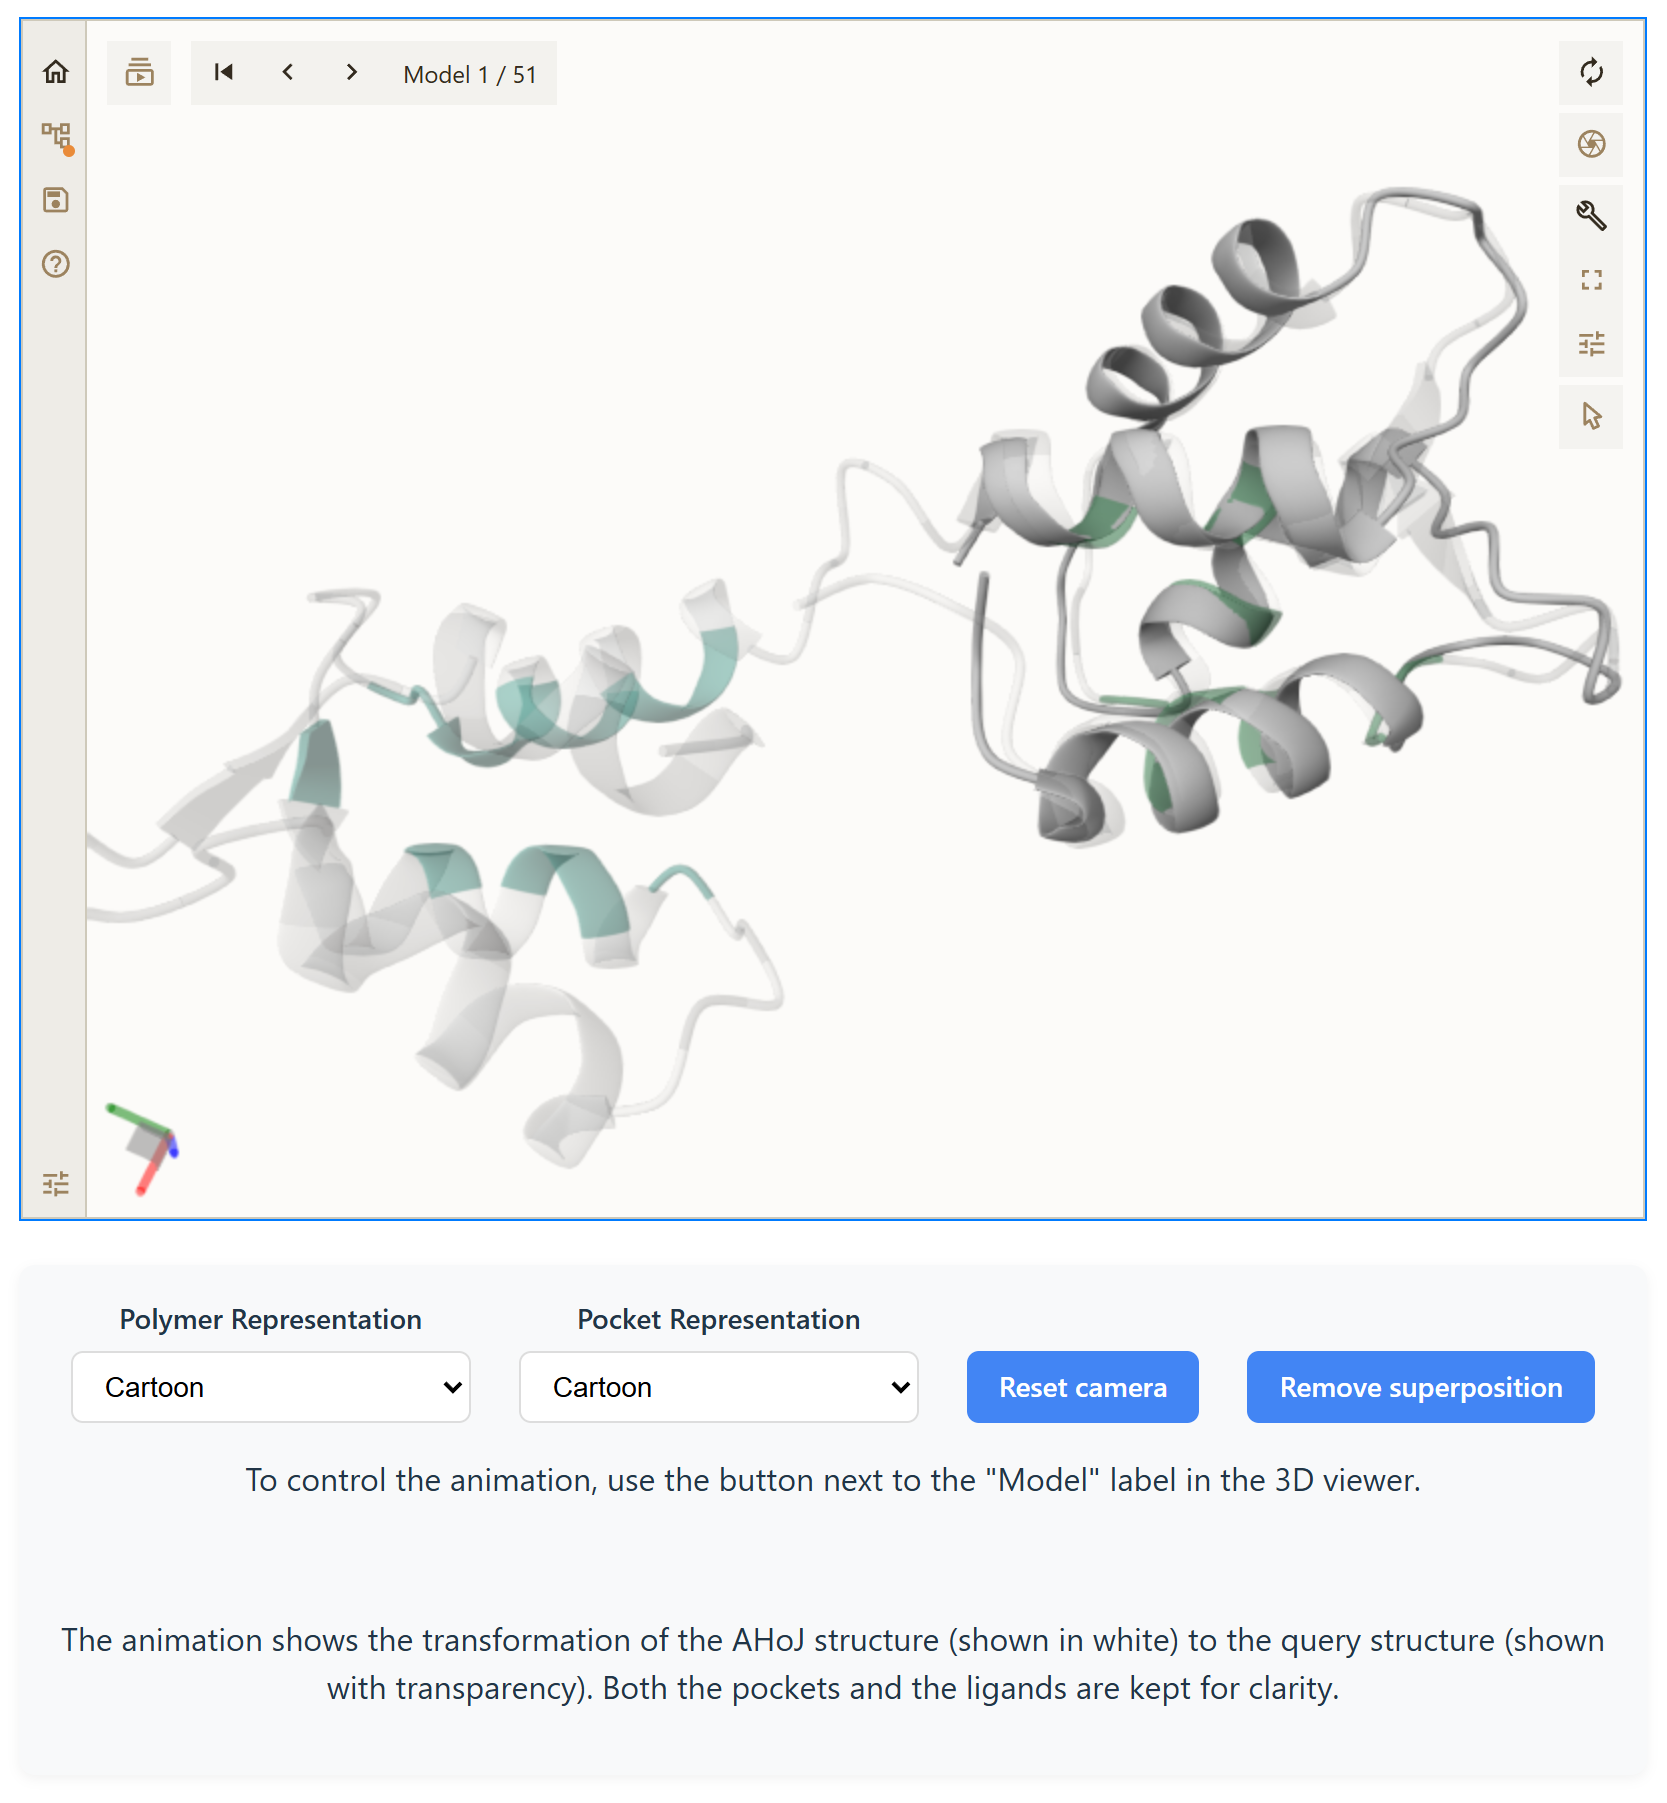
\includegraphics[width=\textwidth]{img/ui-molstar.png}
    \caption{Mol* 3D visualization of the protein structure of Calcium-free Calmodulin (1CFD), along with the Crystal Structure of Myosin-1c tail in complex with Calmodulin (4R8G), with the visualization toolbox underneath.}
    \label{fig:ui-molstar}
\end{figure}

\begin{figure}[htbp]
    \centering
    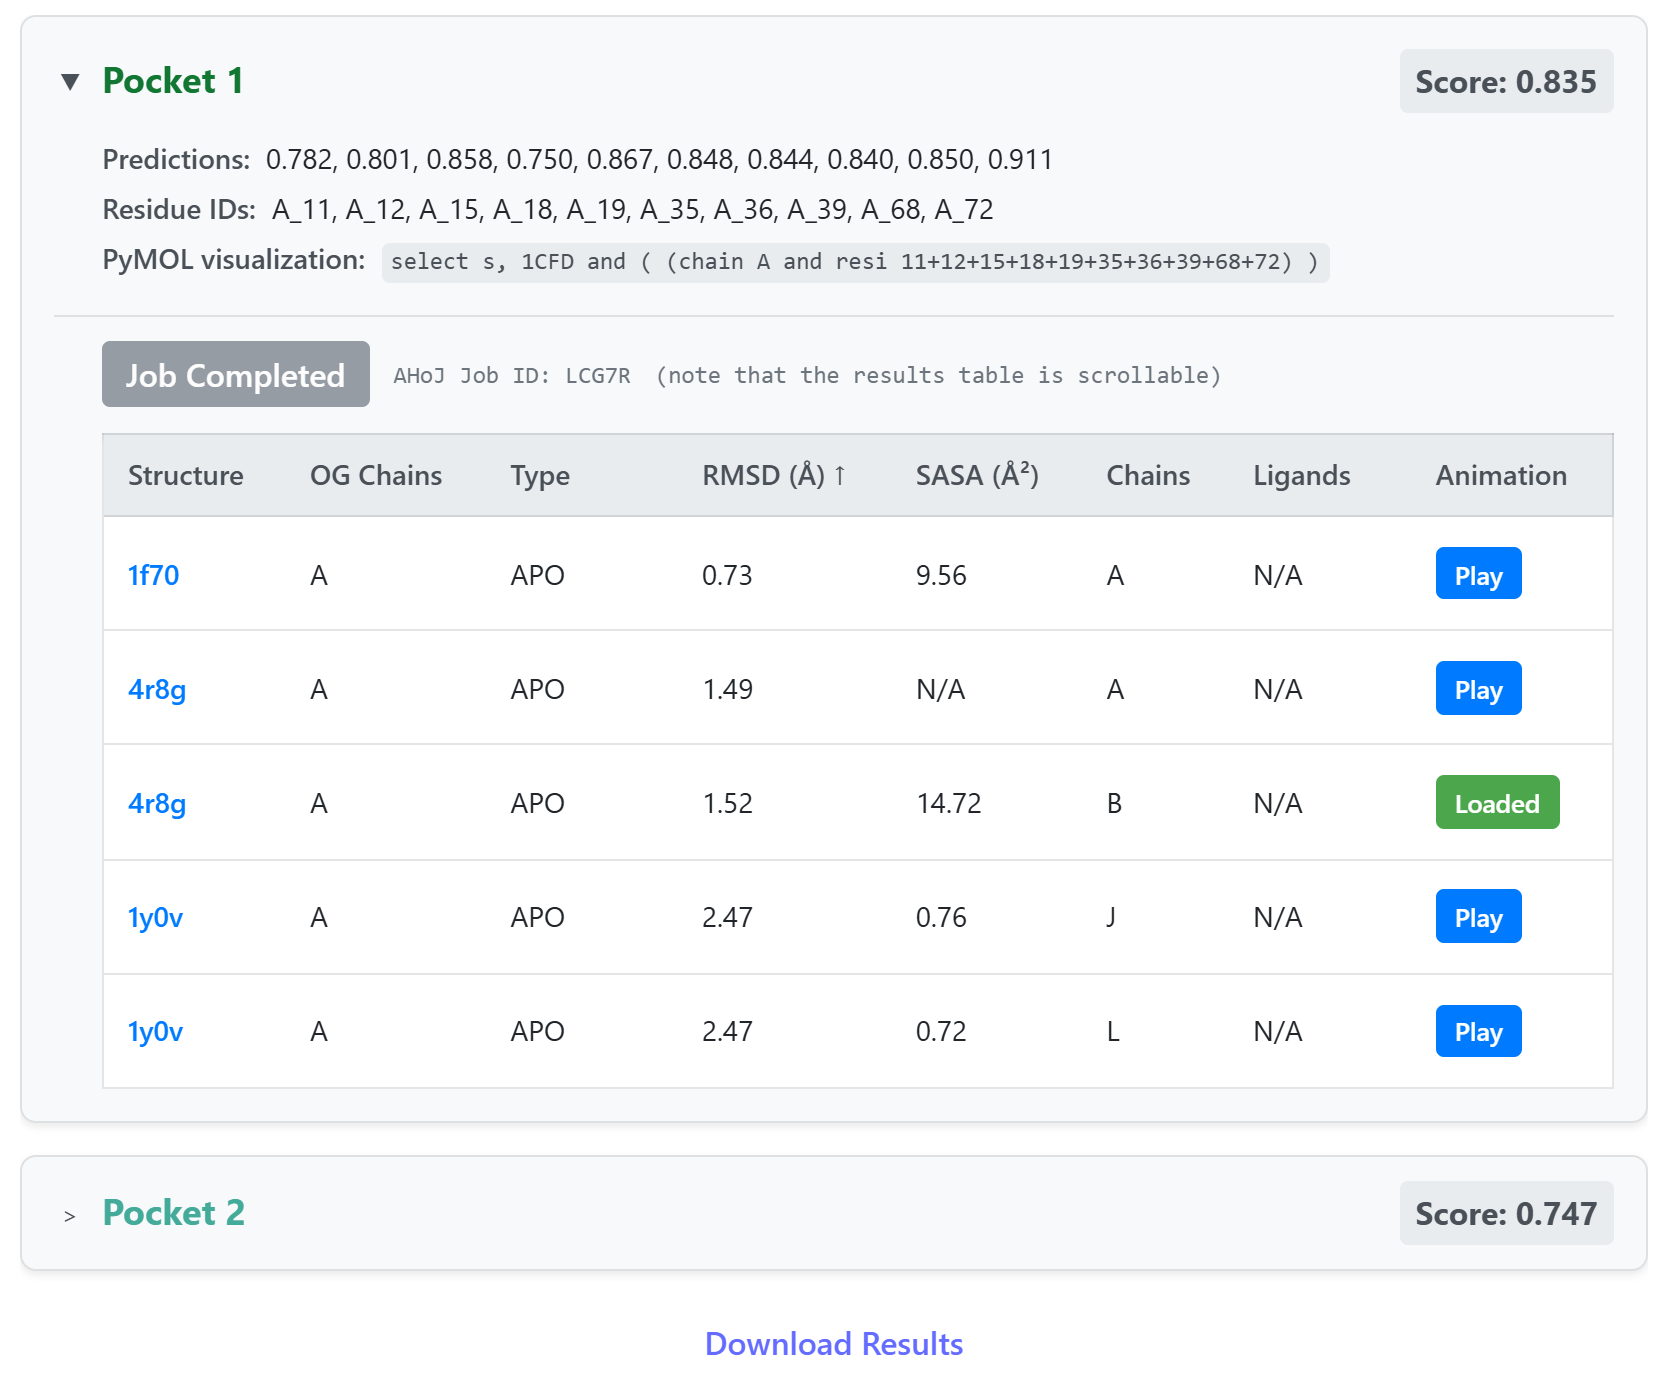
\includegraphics[width=\textwidth]{img/ui-table.png}
    \caption{Table of cryptic binding sites for the Calcium-free Calmodulin (1CFD) protein structure with expandable rows, showing details about the involved residues, their scores, and a PyMOL selection string for visualizing the site in PyMOL.}
    \label{fig:ui-table}
\end{figure}

\section{Use Case: Predicting Cryptic Binding Sites in DHFR}
\label{sec:use-case}

To illustrate the intended use of the CryptoShow application, we examine a real-world example from computational drug discovery. This scenario demonstrates how structural analysis and simulation tools can uncover cryptic binding sites in proteins—sites that are not evident in ligand-free structures but emerge in ligand-bound forms or during dynamic conformational changes. This example is inspired by the work of \citet{meller2023predicting}.

\subsection{Case Study: Dihydrofolate Reductase (DHFR)}
\label{subsec:dhfr-example}

As a case study, we use the protein dihydrofolate reductase (DHFR) from \textit{Escherichia coli}, an important target in antimicrobial drug development \cite{heaslet2009structural}. We begin with the apo structure, PDB ID \textbf{2W9T}, which shows DHFR in its unbound state with no visible deep binding pockets beyond the known active site.

Using the CryptoShow application, we predict potential cryptic pockets based solely on the apo structure. One binding site is identified near the so-called Met20 loop\footnote{The Met20 loop is a flexible segment of DHFR, named after the methionine amino acid at position 20 (residue ID 42 in this structure), and is known for its role in modulating access to the active site through conformational changes.}, a flexible region of the protein known to undergo conformational changes. The prediction is shown in Figure~\ref{fig:ui-cryptic-pocket}.

\begin{figure}[htbp]
    \centering
    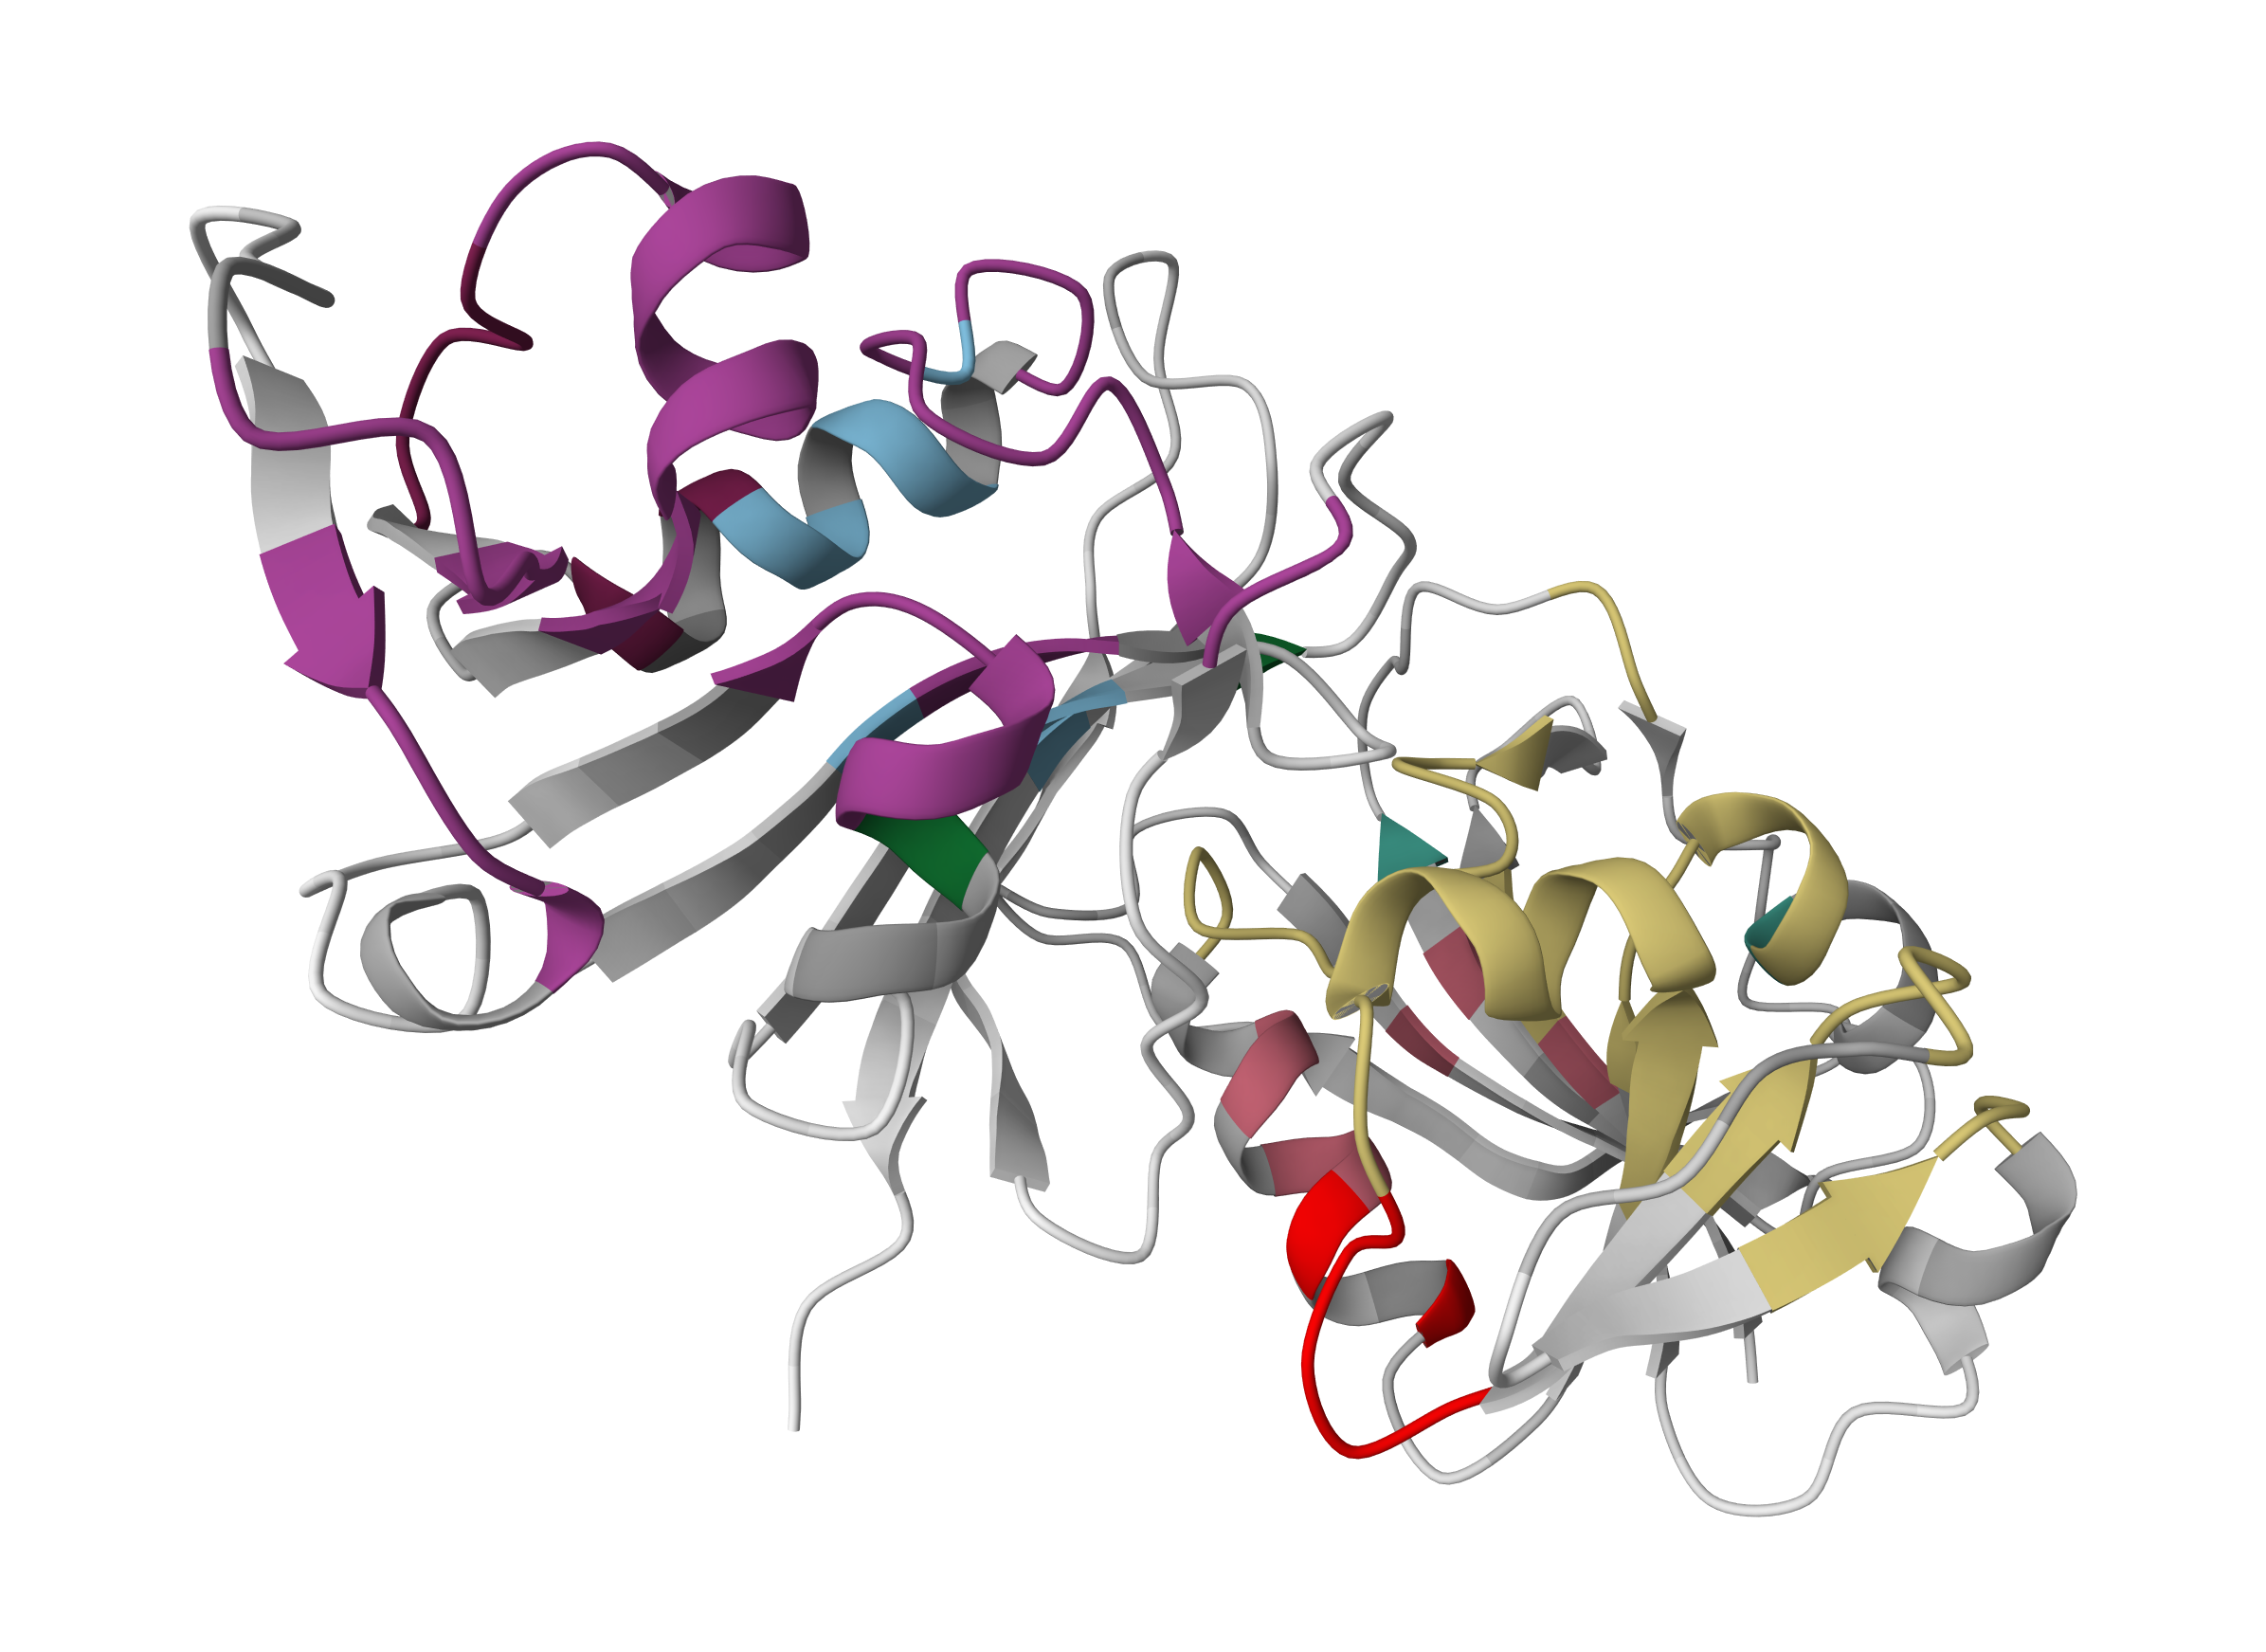
\includegraphics[width=\textwidth]{img/2w9t_prediction.png}
    \caption{Predicted cryptic binding sites in the apo structure of DHFR (PDB ID 2W9T) using the CryptoShow application. The pockets are highlighted in different colors, with the Met20 binding site shown in light yellow. Visualized using Mol*.}
    \label{fig:ui-cryptic-pocket}
\end{figure}

\subsection{Validation Using Holo Structure}
\label{subsec:holo-validation}

To evaluate the accuracy of the prediction, we consult the AHoJ database to identify known holo structures of DHFR. Indeed, a holo form is available: PDB ID \textbf{2W9S}, in which the protein is bound to the antimicrobial drug Trimethoprim. In this structure, the Met20 loop shifts position, exposing a pocket that matches the one predicted by the CryptoShow application from the apo form. The conformational change of the Met20 loop can be visualized in the application.

This comparison between 2W9T (apo) and 2W9S (holo) provides a validation of the cryptic pocket prediction. The application was able to identify a site that is not visible in the apo structure but becomes occupied by a ligand in the holo structure.

\subsection{Further Exploration via Molecular Dynamics}
\label{subsec:md-exploration}

To further investigate the dynamic opening of the predicted pocket, one can perform molecular dynamics (MD) simulations using tools such as GROMACS~\cite{van2005gromacs}, starting from the 2W9T structure. While CryptoShow provides only a brief, illustrative visualization of the conformational change, MD simulations offer a detailed and realistic exploration of the protein's dynamics. During the simulation, the Met20 loop displays conformational flexibility, and the predicted pocket transiently appears. Pocket detection tools such as Fpocket~\cite{le2009fpocket} and TRAPP~\cite{kokh2013trapp} can be used to monitor the pocket's volume and accessibility throughout the simulation.

The results support the idea that the site is not an artifact of ligand binding, but a real conformational feature that may be exploited for inhibitor design and further studies.

\subsection{Use Case Conclusion}
\label{subsec:use-case-conclusion}

This use case demonstrates how the CryptoShow application can be used to predict cryptic binding sites from an apo structure, and how known holo structures, such as 2W9S, can be used to validate the accuracy of those predictions. It highlights the practical application of structural bioinformatics and simulation tools in supporting early-stage drug discovery efforts, demonstrating the real-world utility of the developed application in computational structural biology research.
